% Options for packages loaded elsewhere
\PassOptionsToPackage{unicode}{hyperref}
\PassOptionsToPackage{hyphens}{url}
%
\documentclass[
]{book}
\usepackage{amsmath,amssymb}
\usepackage{lmodern}
\usepackage{iftex}
\ifPDFTeX
  \usepackage[T1]{fontenc}
  \usepackage[utf8]{inputenc}
  \usepackage{textcomp} % provide euro and other symbols
\else % if luatex or xetex
  \usepackage{unicode-math}
  \defaultfontfeatures{Scale=MatchLowercase}
  \defaultfontfeatures[\rmfamily]{Ligatures=TeX,Scale=1}
\fi
% Use upquote if available, for straight quotes in verbatim environments
\IfFileExists{upquote.sty}{\usepackage{upquote}}{}
\IfFileExists{microtype.sty}{% use microtype if available
  \usepackage[]{microtype}
  \UseMicrotypeSet[protrusion]{basicmath} % disable protrusion for tt fonts
}{}
\makeatletter
\@ifundefined{KOMAClassName}{% if non-KOMA class
  \IfFileExists{parskip.sty}{%
    \usepackage{parskip}
  }{% else
    \setlength{\parindent}{0pt}
    \setlength{\parskip}{6pt plus 2pt minus 1pt}}
}{% if KOMA class
  \KOMAoptions{parskip=half}}
\makeatother
\usepackage{xcolor}
\IfFileExists{xurl.sty}{\usepackage{xurl}}{} % add URL line breaks if available
\IfFileExists{bookmark.sty}{\usepackage{bookmark}}{\usepackage{hyperref}}
\hypersetup{
  pdftitle={Bayesian latent class models for prevalence estimation and diagnostic test evaluation},
  pdfauthor={Simon Dufour and Juan Carlos Arango Sabogal},
  hidelinks,
  pdfcreator={LaTeX via pandoc}}
\urlstyle{same} % disable monospaced font for URLs
\usepackage{color}
\usepackage{fancyvrb}
\newcommand{\VerbBar}{|}
\newcommand{\VERB}{\Verb[commandchars=\\\{\}]}
\DefineVerbatimEnvironment{Highlighting}{Verbatim}{commandchars=\\\{\}}
% Add ',fontsize=\small' for more characters per line
\usepackage{framed}
\definecolor{shadecolor}{RGB}{248,248,248}
\newenvironment{Shaded}{\begin{snugshade}}{\end{snugshade}}
\newcommand{\AlertTok}[1]{\textcolor[rgb]{0.94,0.16,0.16}{#1}}
\newcommand{\AnnotationTok}[1]{\textcolor[rgb]{0.56,0.35,0.01}{\textbf{\textit{#1}}}}
\newcommand{\AttributeTok}[1]{\textcolor[rgb]{0.77,0.63,0.00}{#1}}
\newcommand{\BaseNTok}[1]{\textcolor[rgb]{0.00,0.00,0.81}{#1}}
\newcommand{\BuiltInTok}[1]{#1}
\newcommand{\CharTok}[1]{\textcolor[rgb]{0.31,0.60,0.02}{#1}}
\newcommand{\CommentTok}[1]{\textcolor[rgb]{0.56,0.35,0.01}{\textit{#1}}}
\newcommand{\CommentVarTok}[1]{\textcolor[rgb]{0.56,0.35,0.01}{\textbf{\textit{#1}}}}
\newcommand{\ConstantTok}[1]{\textcolor[rgb]{0.00,0.00,0.00}{#1}}
\newcommand{\ControlFlowTok}[1]{\textcolor[rgb]{0.13,0.29,0.53}{\textbf{#1}}}
\newcommand{\DataTypeTok}[1]{\textcolor[rgb]{0.13,0.29,0.53}{#1}}
\newcommand{\DecValTok}[1]{\textcolor[rgb]{0.00,0.00,0.81}{#1}}
\newcommand{\DocumentationTok}[1]{\textcolor[rgb]{0.56,0.35,0.01}{\textbf{\textit{#1}}}}
\newcommand{\ErrorTok}[1]{\textcolor[rgb]{0.64,0.00,0.00}{\textbf{#1}}}
\newcommand{\ExtensionTok}[1]{#1}
\newcommand{\FloatTok}[1]{\textcolor[rgb]{0.00,0.00,0.81}{#1}}
\newcommand{\FunctionTok}[1]{\textcolor[rgb]{0.00,0.00,0.00}{#1}}
\newcommand{\ImportTok}[1]{#1}
\newcommand{\InformationTok}[1]{\textcolor[rgb]{0.56,0.35,0.01}{\textbf{\textit{#1}}}}
\newcommand{\KeywordTok}[1]{\textcolor[rgb]{0.13,0.29,0.53}{\textbf{#1}}}
\newcommand{\NormalTok}[1]{#1}
\newcommand{\OperatorTok}[1]{\textcolor[rgb]{0.81,0.36,0.00}{\textbf{#1}}}
\newcommand{\OtherTok}[1]{\textcolor[rgb]{0.56,0.35,0.01}{#1}}
\newcommand{\PreprocessorTok}[1]{\textcolor[rgb]{0.56,0.35,0.01}{\textit{#1}}}
\newcommand{\RegionMarkerTok}[1]{#1}
\newcommand{\SpecialCharTok}[1]{\textcolor[rgb]{0.00,0.00,0.00}{#1}}
\newcommand{\SpecialStringTok}[1]{\textcolor[rgb]{0.31,0.60,0.02}{#1}}
\newcommand{\StringTok}[1]{\textcolor[rgb]{0.31,0.60,0.02}{#1}}
\newcommand{\VariableTok}[1]{\textcolor[rgb]{0.00,0.00,0.00}{#1}}
\newcommand{\VerbatimStringTok}[1]{\textcolor[rgb]{0.31,0.60,0.02}{#1}}
\newcommand{\WarningTok}[1]{\textcolor[rgb]{0.56,0.35,0.01}{\textbf{\textit{#1}}}}
\usepackage{longtable,booktabs,array}
\usepackage{calc} % for calculating minipage widths
% Correct order of tables after \paragraph or \subparagraph
\usepackage{etoolbox}
\makeatletter
\patchcmd\longtable{\par}{\if@noskipsec\mbox{}\fi\par}{}{}
\makeatother
% Allow footnotes in longtable head/foot
\IfFileExists{footnotehyper.sty}{\usepackage{footnotehyper}}{\usepackage{footnote}}
\makesavenoteenv{longtable}
\usepackage{graphicx}
\makeatletter
\def\maxwidth{\ifdim\Gin@nat@width>\linewidth\linewidth\else\Gin@nat@width\fi}
\def\maxheight{\ifdim\Gin@nat@height>\textheight\textheight\else\Gin@nat@height\fi}
\makeatother
% Scale images if necessary, so that they will not overflow the page
% margins by default, and it is still possible to overwrite the defaults
% using explicit options in \includegraphics[width, height, ...]{}
\setkeys{Gin}{width=\maxwidth,height=\maxheight,keepaspectratio}
% Set default figure placement to htbp
\makeatletter
\def\fps@figure{htbp}
\makeatother
\setlength{\emergencystretch}{3em} % prevent overfull lines
\providecommand{\tightlist}{%
  \setlength{\itemsep}{0pt}\setlength{\parskip}{0pt}}
\setcounter{secnumdepth}{-\maxdimen} % remove section numbering
\usepackage{booktabs}
\usepackage{longtable}
\usepackage{array}
\usepackage{multirow}
\usepackage{wrapfig}
\usepackage{float}
\usepackage{colortbl}
\usepackage{pdflscape}
\usepackage{tabu}
\usepackage{threeparttable}
\usepackage{threeparttablex}
\usepackage[normalem]{ulem}
\usepackage{makecell}
\usepackage{xcolor}
\ifLuaTeX
  \usepackage{selnolig}  % disable illegal ligatures
\fi

\title{Bayesian latent class models for prevalence estimation and
diagnostic test evaluation}
\author{Simon Dufour and Juan Carlos Arango Sabogal}
\date{2022-05-04}

\begin{document}
\frontmatter
\maketitle

\mainmatter
\begin{figure}
\centering

\includegraphics{Figures/national-cancer-institute-NFvdKIhxYlU-unsplash.jpg}
\caption{Credit: National Cancer Institute on Unsplash}
\end{figure}

\hypertarget{about-this-document}{%
\chapter{About this document}\label{about-this-document}}

In this document you will find indications on how to use various
\texttt{R} libraries and functions for estimating true disease
prevalence and accuracy of diagnostic tests in a Bayesian framework,
along with various exercises. We suppose that you do have some basic
\texttt{R} skills. If you have not worked with \texttt{R} before or feel
a bit rusty, here are some resources to help you to prepare:

\begin{itemize}
\item
  Chapters 1, 2, and 4 of the
  \href{https://www.codecademy.com/learn/learn-r}{CodeCademy ``Learn R''
  course} will provide a good overview of the basic concepts required
  for this workshop.
\item
  If you are familiar with \texttt{R} and want to do some further
  reading, \href{https://r4ds.had.co.nz/}{Hadley Wickham's ``R for Data
  Science''} is a great resource.
\end{itemize}

Remember, there are often many different ways to conduct a given piece
of work in \texttt{R}. Throughout this document, we tried to stick with
the simpler approaches (e.g., the shortest code, the minimal number of
\texttt{R} libraries).

\hypertarget{some-notation}{%
\section{Some notation}\label{some-notation}}

Throughout the document, you will find examples of \texttt{R} code along
with comments. \textbf{The \texttt{R} code used always appear in grey
boxes} (see the following example). This is the code that you will be
able to use for your own analyses. \textbf{Lines that are preceded by a
\# sign are comments}, they are skipped when \texttt{R} reads them.
Following each grey box with \texttt{R} code, a \textbf{white box with
results from the analysis is presented}.

For instance, this is a \texttt{R} code where I am simply asking to show
main descriptive statistics for the \emph{speed} variable of the
\emph{cars} dataset (note that this dataset is already part of
\texttt{R}).

\begin{Shaded}
\begin{Highlighting}[]
\CommentTok{\#This is a comment. R will ignore this line}

\CommentTok{\#The summary() function can be use to ask for a summary of various R objects. For a variable (here the variable speed), it shows descriptive statistics.}
\FunctionTok{summary}\NormalTok{(cars}\SpecialCharTok{$}\NormalTok{speed)}
\end{Highlighting}
\end{Shaded}

\begin{verbatim}
##    Min. 1st Qu.  Median    Mean 3rd Qu.    Max. 
##     4.0    12.0    15.0    15.4    19.0    25.0
\end{verbatim}

Throughout the document, in the text I will use:\\
- Italics for datasets or variables. For instance, the \emph{speed}
variable of the dataset \emph{cars}.\\
- Shaded boxes for \texttt{R} libraries (e.g., \texttt{episensr}) and
functions (e.g., \texttt{summary()}).

In \texttt{R} we can first call a given library and then use the
functions related to each library or we can name the library followed by
\texttt{::} and then the function. For instance the two following pieces
of code are equivalent:

\begin{Shaded}
\begin{Highlighting}[]
\FunctionTok{library}\NormalTok{(ggplot2)}
\FunctionTok{ggplot}\NormalTok{(}\AttributeTok{data=}\NormalTok{cars, }\AttributeTok{mapping=}\NormalTok{(}\FunctionTok{aes}\NormalTok{(}\AttributeTok{x=}\NormalTok{speed)))}\SpecialCharTok{+}
  \FunctionTok{geom\_histogram}\NormalTok{()}

\DocumentationTok{\#\#OR\#\#}

\NormalTok{ggplot2}\SpecialCharTok{::}\FunctionTok{ggplot}\NormalTok{(}\AttributeTok{data=}\NormalTok{cars, }\AttributeTok{mapping=}\NormalTok{(}\FunctionTok{aes}\NormalTok{(}\AttributeTok{x=}\NormalTok{speed)))}\SpecialCharTok{+}
  \FunctionTok{geom\_histogram}\NormalTok{()}
\end{Highlighting}
\end{Shaded}

The latter may improve reproducibility, but to the expense of longer
codes. Throughout the document, we will always first call the library
and then run the functions to keep codes shorter.

One last thing, when using a given function, it is not mandatory to name
all the arguments, as long as they are presented in the sequence
expected by this function. For instance, the \texttt{ggplot()} function
that we used in the previous chunk of code is expecting to see first a
dataset (\texttt{data=}) and then a mapping attribute
(\texttt{mapping=}) and, within that mapping attribute a x variable
(\texttt{x=}). We could shorten the code by omitting all of these. The
two following pieces of code are, therefore, equivalent:

\begin{Shaded}
\begin{Highlighting}[]
\FunctionTok{library}\NormalTok{(ggplot2)}
\FunctionTok{ggplot}\NormalTok{(}\AttributeTok{data=}\NormalTok{cars, }\AttributeTok{mapping=}\NormalTok{(}\FunctionTok{aes}\NormalTok{(}\AttributeTok{x=}\NormalTok{speed)))}\SpecialCharTok{+}
  \FunctionTok{geom\_histogram}\NormalTok{()}

\DocumentationTok{\#\#OR\#\#  }

\FunctionTok{library}\NormalTok{(ggplot2)}
\FunctionTok{ggplot}\NormalTok{(cars, (}\FunctionTok{aes}\NormalTok{(speed)))}\SpecialCharTok{+}
  \FunctionTok{geom\_histogram}\NormalTok{()}
\end{Highlighting}
\end{Shaded}

Throughout the document, however, we will use the longer code with all
the arguments being named. Since you are learning these new functions,
it would be quite a challenge to use the shorter code right from the
start. But you could certainly adopt the shorter codes later on.

\textbf{LET'S GET STARTED!}

\hypertarget{distributions}{%
\chapter{Distributions}\label{distributions}}

When using latent class models (LCM) to estimate disease prevalence or
diagnostic test accuracy, we will need to use various distributions.
There are two situations where we will use distributions:

\begin{enumerate}
\def\labelenumi{\arabic{enumi})}
\tightlist
\item
  as prior distribution to describe our a priori knowledge on a given
  unknown parameter.\\
\item
  as a part of the likelihood function that will be used to linked
  observed data with unknown parameters.
\end{enumerate}

Some distributions will more often be used for the first objective,
others will mainly be used for the latter objective. In he following
sections, we will cover the most usefull distributions.

\hypertarget{prior-distributions}{%
\section{Prior distributions}\label{prior-distributions}}

One of the first thing that you will need for any Bayesian analysis is a
way to generate and visualize a prior distribution corresponding to some
scientific knowledge that you have about an unknown parameter.
Generally, you will use information such as the mean and variance or the
mode and the 2.5th (or 97.5th) percentile to find a corresponding
distribution. You will use various distributions. Here is a list of the
most important ones, we will give more details on each of them in the
following sections:

\textbf{- Normal distribution:} defined by a mean (mu) and its standard
deviation (SD) or variance (tau). In some packages and software,
\texttt{rjags} and JAGS for instance, the inverse of the variance
(1/tau) is used to specify a given normal distribution.\\
\textbf{Notation: dNorm(mu, 1/tau)}

\textbf{- Uniform distribution:} defined by a minimum (min) and maximum
(max).\\
\textbf{Notation: dUnif(min, max)}

\textbf{- Beta distribution:} bounded between 0 and 1, beta
distributions are defined by two shape parameters (a) and (b).\\
\textbf{Notation: dBeta(a, b)}

\hypertarget{normal-distribution}{%
\subsection{Normal distribution}\label{normal-distribution}}

The \texttt{dnorm()} function can be used to generate a given Normal
distribution and the \texttt{curve()} function can be used to visualize
the generated distribution. These functions are already part of
\texttt{R}, there is no need to upload a \texttt{R} package.

\begin{Shaded}
\begin{Highlighting}[]
\FunctionTok{curve}\NormalTok{(}\FunctionTok{dnorm}\NormalTok{(x, }\AttributeTok{mean=}\FloatTok{2.0}\NormalTok{, }\AttributeTok{sd=}\FloatTok{0.5}\NormalTok{),                                    }\CommentTok{\# I indicate mean and SD of the distribution}
      \AttributeTok{from=}\SpecialCharTok{{-}}\DecValTok{2}\NormalTok{, }\AttributeTok{to=}\DecValTok{7}\NormalTok{,                                                 }\CommentTok{\# I indicate limits for the plot}
      \AttributeTok{main=}\StringTok{"Normal distribution with mean of 2.0 and SD of 0.5"}\NormalTok{,     }\CommentTok{\#Adding a title}
      \AttributeTok{xlab =} \StringTok{"Value"}\NormalTok{, }\AttributeTok{ylab =} \StringTok{"Density"}\NormalTok{)                              }\CommentTok{\#Adding titles for axes}
\end{Highlighting}
\end{Shaded}

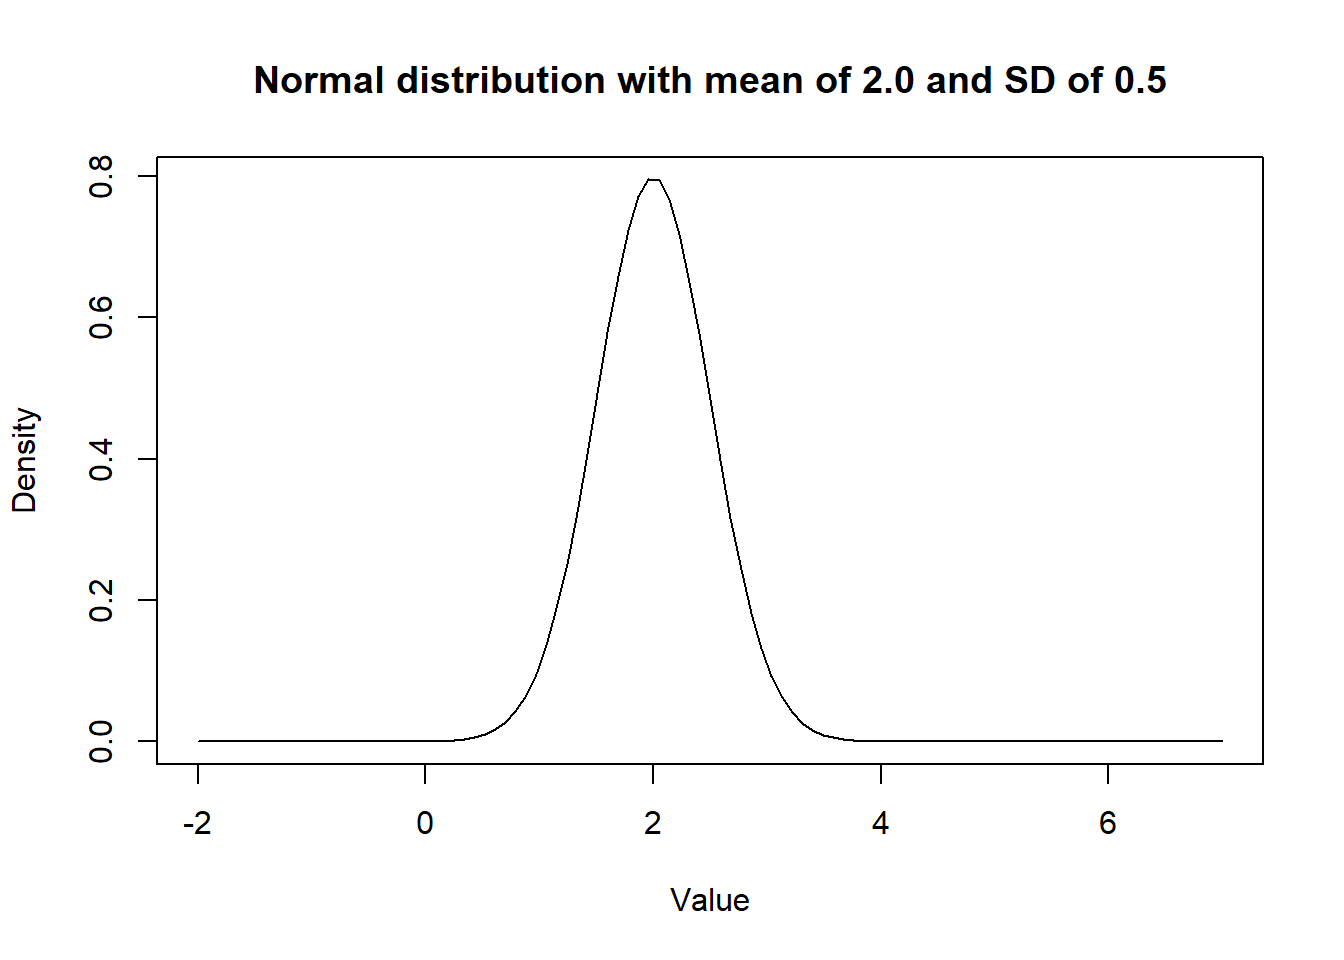
\includegraphics{_main_files/figure-latex/unnamed-chunk-4-1.pdf} Note
that a Normal distribution with mean of zero and a very large SD
provides very little information. Such distribution would be referred to
as a \textbf{uniform or flat distribution} (A.K.A.; a vague
distribution).

\begin{Shaded}
\begin{Highlighting}[]
\FunctionTok{curve}\NormalTok{(}\FunctionTok{dnorm}\NormalTok{(x, }\AttributeTok{mean=}\FloatTok{0.0}\NormalTok{, }\AttributeTok{sd=}\DecValTok{10000000000}\NormalTok{),                                    }
      \AttributeTok{from=}\SpecialCharTok{{-}}\DecValTok{100}\NormalTok{, }\AttributeTok{to=}\DecValTok{100}\NormalTok{,                                                 }
      \AttributeTok{main=}\StringTok{"A flat Normal distribution"}\NormalTok{,     }
      \AttributeTok{xlab =} \StringTok{"Value"}\NormalTok{, }\AttributeTok{ylab =} \StringTok{"Density"}\NormalTok{)                              }
\end{Highlighting}
\end{Shaded}

\begin{figure}
\centering
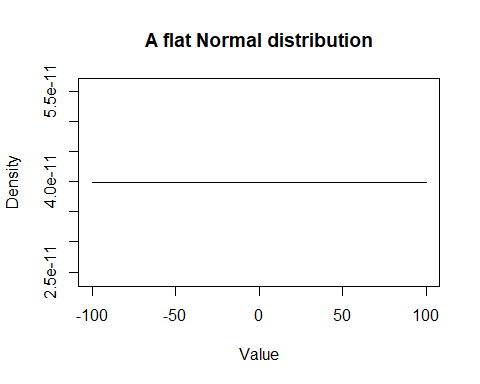
\includegraphics{_main_files/figure-latex/unnamed-chunk-5-1.pdf}
\caption{Density curve of a flat Normal distribution.}
\end{figure}

\hypertarget{uniform-distribution}{%
\subsection{Uniform distribution}\label{uniform-distribution}}

In the same manner, we could visualize an uniform distribution using the
\texttt{dunif()} function. In the following example, we assumed that any
values between -5.0 and 5.0 are equally probable.

\begin{Shaded}
\begin{Highlighting}[]
\FunctionTok{curve}\NormalTok{(}\FunctionTok{dunif}\NormalTok{(x, }\AttributeTok{min=}\SpecialCharTok{{-}}\FloatTok{5.0}\NormalTok{, }\AttributeTok{max=}\FloatTok{5.0}\NormalTok{),                                    }
      \AttributeTok{from=}\SpecialCharTok{{-}}\DecValTok{10}\NormalTok{, }\AttributeTok{to=}\DecValTok{10}\NormalTok{,                                                 }
      \AttributeTok{main=}\StringTok{"Uniform distribution with {-}5.0 and 5.0 limits"}\NormalTok{,    }
      \AttributeTok{xlab =} \StringTok{"Value"}\NormalTok{, }\AttributeTok{ylab =} \StringTok{"Density"}\NormalTok{)                              }
\end{Highlighting}
\end{Shaded}

\begin{figure}
\centering
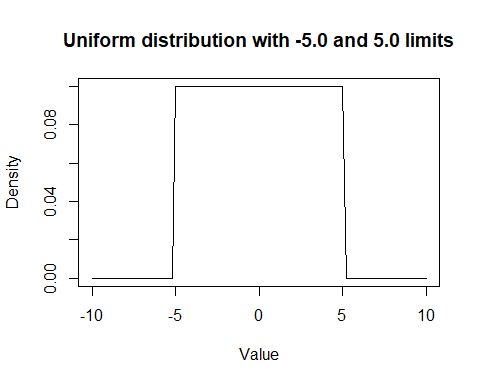
\includegraphics{_main_files/figure-latex/unnamed-chunk-6-1.pdf}
\caption{Density curve of an Uniform distribution.}
\end{figure}

\hypertarget{beta-distribution}{%
\subsection{Beta distribution}\label{beta-distribution}}

Beta distributions are another type of distributions that will
specifically be used for parameters that are proportions (i.e., bounded
between 0.0 and 1.0). For this specific workshop, they will be very
handy, since a sensitivity, specificity, or a prevalence are all
proportions . The \texttt{epi.betabuster()} function from the
\texttt{epiR} library can be used to define a given prior distribution
based on previous knowledge. When you use the \texttt{epi.betabuster()}
function, it creates a new \texttt{R} object containing different
elements. Among these, one element will be named \emph{shape1} and
another \emph{shape2}. These correspond to the a and b shape parameters
of the corresponding Beta distribution.

For instance we may know that the most likely value for the sensitivity
of a given test is 0.85 and that we are 97.5\% certain that it is
greater than 0.75. With these values, we will be able to find the a and
b shape parameters of the corresponding Beta distribution.

\begin{Shaded}
\begin{Highlighting}[]
\FunctionTok{library}\NormalTok{(epiR) }

\CommentTok{\# Sensitivity of a test as Mode=0.85, and we are 97.5\% sure \textgreater{}0.75 }
\NormalTok{rval }\OtherTok{\textless{}{-}} \FunctionTok{epi.betabuster}\NormalTok{(}\AttributeTok{mode=}\FloatTok{0.85}\NormalTok{, }\AttributeTok{conf=}\FloatTok{0.975}\NormalTok{, }\AttributeTok{greaterthan=}\NormalTok{T, }\AttributeTok{x=}\FloatTok{0.75}\NormalTok{)  }\CommentTok{\# I create a new object named rval}

\NormalTok{rval}\SpecialCharTok{$}\NormalTok{shape1                }\CommentTok{\#View the a shape parameter in rval}
\end{Highlighting}
\end{Shaded}

\begin{verbatim}
## [1] 62.661
\end{verbatim}

\begin{Shaded}
\begin{Highlighting}[]
\NormalTok{rval}\SpecialCharTok{$}\NormalTok{shape2                }\CommentTok{\#View the b shape parameter in rval  }
\end{Highlighting}
\end{Shaded}

\begin{verbatim}
## [1] 11.88135
\end{verbatim}

\begin{Shaded}
\begin{Highlighting}[]
\CommentTok{\#plot the prior distribution}
\FunctionTok{curve}\NormalTok{(}\FunctionTok{dbeta}\NormalTok{(x, }\AttributeTok{shape1=}\NormalTok{rval}\SpecialCharTok{$}\NormalTok{shape1, }\AttributeTok{shape2=}\NormalTok{rval}\SpecialCharTok{$}\NormalTok{shape2), }\AttributeTok{from=}\DecValTok{0}\NormalTok{, }\AttributeTok{to=}\DecValTok{1}\NormalTok{, }
      \AttributeTok{main=}\StringTok{"Prior for test\textquotesingle{}s sensitivity"}\NormalTok{, }\AttributeTok{xlab =} \StringTok{"Proportion"}\NormalTok{, }\AttributeTok{ylab =} \StringTok{"Density"}\NormalTok{)}
\end{Highlighting}
\end{Shaded}

\begin{figure}
\centering
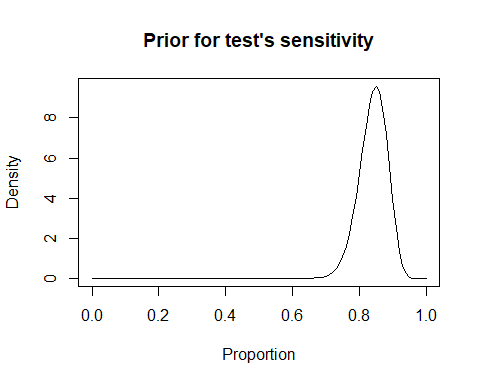
\includegraphics{_main_files/figure-latex/unnamed-chunk-7-1.pdf}
\caption{Density curve of a Beta distribution for a test sensitivity.}
\end{figure}

Note that a dBeta(1.0, 1.0) is a uniform beta distribution.

\begin{Shaded}
\begin{Highlighting}[]
\CommentTok{\#plot the prior distribution}
\FunctionTok{curve}\NormalTok{(}\FunctionTok{dbeta}\NormalTok{(x, }\AttributeTok{shape1=}\FloatTok{1.0}\NormalTok{, }\AttributeTok{shape2=}\FloatTok{1.0}\NormalTok{), }\AttributeTok{from=}\DecValTok{0}\NormalTok{, }\AttributeTok{to=}\DecValTok{1}\NormalTok{, }
      \AttributeTok{main=}\StringTok{"A Beta(1.0, 1.0) or flat distribution"}\NormalTok{, }\AttributeTok{xlab =} \StringTok{"Proportion"}\NormalTok{, }\AttributeTok{ylab =} \StringTok{"Density"}\NormalTok{)}
\end{Highlighting}
\end{Shaded}

\begin{figure}
\centering
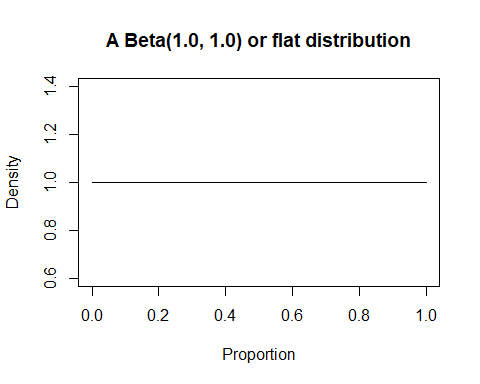
\includegraphics{_main_files/figure-latex/unnamed-chunk-8-1.pdf}
\caption{Density curve of a Beta(1.0, 1.0) distribution.}
\end{figure}

\hypertarget{distributions-for-likelihood-functions}{%
\section{Distributions for likelihood
functions}\label{distributions-for-likelihood-functions}}

In many situations, a distribution will be used as a part of the
likelihood function to link observed data to unknown parameters. The
ones we will most frequently used here are:

\textbf{- Binomial distribution:} For variables that can take the value
0 or 1. Binomial distributions are defined by a probability, P, which is
the probability that the variable takes the value 1, and a number of
``trials'', n.\\
\textbf{Notation: dBin(P, n)}

\textbf{- Multinomial distribution:} made up of a number of
probabilities, all bounded between 0 and 1, and that, together, will sum
up to 1. Multinomial distributions are defined by k probabilities (P1,
P2, \ldots, Pk) and a number of observation (n).\\
\textbf{Notation: dmulti(P{[}1:k{]}, n)}

\hypertarget{binomial-distribution}{%
\subsection{Binomial distribution}\label{binomial-distribution}}

If we have a variable that can take only two values, healthy or diseased
(0 or 1), we can estimates an unknown parameter such as the proportion
(P) of diseased individuals (i.e., the disease prevalence), based on the
observed data (a number of positive individuals, T AND a total number of
individuals, n). For instance, if we had 30 diseased (T = 30) out of 100
tested individuals (n=100) we could estimate the unknown parameter P
using this very simple likelihood function:

\(T \sim dbin(P, n)\)

\hypertarget{multinomial-distribution}{%
\subsection{Multinomial distribution}\label{multinomial-distribution}}

A last type of distribution that we will use in our LCM is the
multinomial distribution. When an outcome is categorical with
\textgreater2 categories, we could use a multinomial distribution to
describe the probability that an individual has the value ``A'', or
``B'', or ``C'', etc. In our context, the main application of this
distribution will be for describing the combined results of two (or more
than two) diagnostic tests. For instance, if we cross-tabulate the
results of Test A and Test B, we have four potential outcomes:

-Test A+ and Test B+ (lets call n1 the number of individuals in that
cell and P1 the probability of falling in that cell)\\
-Test A+ and Test B- (n2 and P2)\\
-Test A- and Test B+ (n3 and P3)\\
-Test A- and Test B- (n4 and P4)

We can illustrate this as follow:

\begin{table}

\caption{\label{tab:unnamed-chunk-10}Cross-classified results from two diagnostic tests}
\centering
\begin{tabular}[t]{l|l|l}
\hline
  & Test A+ & Test A-\\
\hline
Test B+ & n1 & n3\\
\hline
Test B- & n2 & n4\\
\hline
\end{tabular}
\end{table}

Thus we could describe the probabilities (P1 to P4) of an individual
falling into one of these cells of the 2x2 table as a multinomial
distribution. In this specific case, we would say that the combined
results of the 2 tests (n1 to n4) and the total number of individual
tested (n), which are the observed data, are linked as follow to the 4
probabilities (P1 to P4; the unknown parameters):

\(n[1:4] \sim dmulti(P[1:4], n)\)

Which means: the values of n1 (or n2, n3, or n4) is determined by the
probability of falling into the ``Test A+ and Test B+'' cell, which is
P1 (or P2, P3, or P4 for the other cells), and by the total number of
individuals tested (n). Nothing too surprising here\ldots{} If I have a
probability of 0.30 to fall in a given cell, and I have tested 100
individuals, I should find 30 individuals in that cell. Wow! Still, the
multinomial distribution is nice because it will ensure that all our
probabilities (P1 to P4) will sum up to exactly 1.0.

\hypertarget{running-bayesian-models}{%
\chapter{Running Bayesian models}\label{running-bayesian-models}}

Different software and \texttt{R} packages can be used to run Bayesian
models. Whether it is a LCM or a more conventional regression model is
not very important at this stage. In this document we will mainly use a
software called JAGS and the \texttt{R2jags} package. So, if not already
done, you will have to download JAGS
\href{https://sourceforge.net/projects/mcmc-jags/files/}{here} and
install it on your computer. Once installed, we will be able to use
\texttt{R2jags} to operate JAGS through \texttt{R}.

Basically, to run any Bayesian model, we will always need the same three
things:

\begin{itemize}
\tightlist
\item
  Data
\item
  A model containing:

  \begin{itemize}
  \tightlist
  \item
    A likelihood function linking observed data to unknown parameters
  \item
    A prior distribution for each unknown parameter
  \end{itemize}
\item
  An initial value for each unknown parameters to start the Markov
  chains

  \begin{itemize}
  \tightlist
  \item
    These values can also be generated randomly by the software, but
    specifying them will improve reproducibility
  \end{itemize}
\end{itemize}

\hypertarget{the-data}{%
\section{The data}\label{the-data}}

This is the easy part. If we were to run, for instance, a
``conventional'' regression analysis, we would have to import in
\texttt{R} a complete dataset (e.g., a CSV file) with a row for each
observation and a column for each variable. However, when using LCM to
estimate a disease prevalence or diagnostic accuracy, the dataset is
simply made up of the number of individuals in each category. For
instance, for estimating a simple prevalence (\emph{Prev}), we could
have 30 individuals that tested positive (variable \emph{T}) out of a
total of 100 individuals (variable \emph{n}). In such case, the dataset
could be created as follow:

\begin{Shaded}
\begin{Highlighting}[]
\CommentTok{\#Creating a dataset}
\NormalTok{datalist }\OtherTok{\textless{}{-}} \FunctionTok{list}\NormalTok{(}\AttributeTok{T=}\DecValTok{30}\NormalTok{, }\AttributeTok{n=}\DecValTok{100}\NormalTok{)}
\end{Highlighting}
\end{Shaded}

If you want to check that it works, you could ask to see this new
\texttt{R} object.

\begin{Shaded}
\begin{Highlighting}[]
\NormalTok{datalist}
\end{Highlighting}
\end{Shaded}

\begin{verbatim}
## $T
## [1] 30
## 
## $n
## [1] 100
\end{verbatim}

\hypertarget{the-model}{%
\section{The model}\label{the-model}}

\hypertarget{the-likelihood-function}{%
\subsection{The likelihood function}\label{the-likelihood-function}}

Lets start with a simple example, estimating a single proportion. For
estimating a proportion we could describe the likelihood function
linking unknown parameters to observed data as follow:

\(T \sim dbin(Prev, n)\)

In other words: the disease prevalence (\emph{Prev}), an unknown
parameter, can be linked to the observed number of positive individuals
(\emph{T}) and the total number of tested individual (\emph{n}) through
the binomial function.

In this case, the values of \emph{T} and \emph{n} are the observed data
and \emph{Prev} is the only unknown parameter.

\hypertarget{priors-for-unkown-parameters}{%
\subsection{Priors for unkown
parameters}\label{priors-for-unkown-parameters}}

We will have to specify a prior distribution for each unknown parameter
(using the \(\sim\) sign).

In the preceding example, we only have one unkown parameter,
\emph{Prev}, which is a proportion. Theoretically such parameter could
take values from 0 to 1, so a beta distribution would be one way to
describe its prior distribution. We could use the
\texttt{epi.betabuster()} function from the \texttt{epiR} library to
define a given beta distribution based on previous knowledge, as
described in the preceding sections. Moreover, if we want to use a flat
prior, we could simply choose the value 1.0 for the a and b shape
parameters.

In the following code, I am creating \texttt{R} objects for a and b for
\emph{Prev} beta prior distributions.

\begin{Shaded}
\begin{Highlighting}[]
\NormalTok{Prev.shapea }\OtherTok{\textless{}{-}} \DecValTok{1}         \CommentTok{\#a shape parameter for Prev    }
\NormalTok{Prev.shapeb }\OtherTok{\textless{}{-}} \DecValTok{1}         \CommentTok{\#b shape parameter for Prev }
\end{Highlighting}
\end{Shaded}

With informative priors, for instance, if we know from the literature
that the prevalence is expected to be 0.25 with 95CI of (0.20, 0.30), we
could instead use the following code and assign these values to
\emph{Prev.shapea} and \emph{Prev.shapeb}:

\begin{Shaded}
\begin{Highlighting}[]
\FunctionTok{library}\NormalTok{(epiR) }

\CommentTok{\# Prevalence as Mode=0.25, and we are 97.5\% sure \textgreater{}0.20 }
\NormalTok{rval }\OtherTok{\textless{}{-}} \FunctionTok{epi.betabuster}\NormalTok{(}\AttributeTok{mode=}\FloatTok{0.25}\NormalTok{, }\AttributeTok{conf=}\FloatTok{0.975}\NormalTok{, }\AttributeTok{greaterthan=}\NormalTok{T, }\AttributeTok{x=}\FloatTok{0.20}\NormalTok{)  }\CommentTok{\# I create a new object named rval}

\NormalTok{rval}\SpecialCharTok{$}\NormalTok{shape1                }\CommentTok{\#View the a shape parameter in rval}
\end{Highlighting}
\end{Shaded}

\begin{verbatim}
## [1] 62.356
\end{verbatim}

\begin{Shaded}
\begin{Highlighting}[]
\NormalTok{rval}\SpecialCharTok{$}\NormalTok{shape2                }\CommentTok{\#View the b shape parameter in rval}
\end{Highlighting}
\end{Shaded}

\begin{verbatim}
## [1] 185.068
\end{verbatim}

\begin{Shaded}
\begin{Highlighting}[]
\CommentTok{\#I left them as comments, but the two lines below would be used to assign the generated values for later usage}
\CommentTok{\#Prev.shapea \textless{}{-} rval$shape1}
\CommentTok{\#Prev.shapeb \textless{}{-} rval$shape2}
\end{Highlighting}
\end{Shaded}

\hypertarget{creating-the-jags-model}{%
\subsection{Creating the JAGS model}\label{creating-the-jags-model}}

Our Bayesian model has to be presented to JAGS as a text file (i.e., a
.txt document). To create this text file, we will use the
\texttt{paste0()} function to write down the model and then the
\texttt{write.table()} function to save it as a .txt file.

\textbf{An interesting feature of the \texttt{paste0()} function is the
possibility to include \texttt{R} objects in the text.} For instance,
you may want to have a general model that will not be modified, but to
change the values used to describe the priors. Within your
\texttt{paste0()} function you could call these ``external'' values.
Thus, you just have to change the value of the \texttt{R} object that
your model is using, rather than rewriting a new model. For instance, we
just created these two \texttt{R} objects called \emph{Prev.shapea} and
\emph{Prev.shapeb} (which were the a and b shape parameters for the
prior distribution of our proportion \emph{Prev}). To describe our prior
distribution, we can ignore this previous work that we have done and
directly create a short text as follow:

\begin{Shaded}
\begin{Highlighting}[]
\NormalTok{text1 }\OtherTok{\textless{}{-}} \FunctionTok{paste0}\NormalTok{(}\StringTok{"Prev \textasciitilde{} dbeta(1, 1)"}\NormalTok{)       }\CommentTok{\#Creating a short text named "text1"}
\NormalTok{text1                                       }\CommentTok{\#Asking to see the text1 object}
\end{Highlighting}
\end{Shaded}

\begin{verbatim}
## [1] "Prev ~ dbeta(1, 1)"
\end{verbatim}

However, if the same model is to be applied later with a different prior
distribution, it may be more convenient to leave the a and b shape
parameters as \texttt{R} objects. Thus, if we change the prior
distribution and run the script again, you would run the entire analyses
with the new distribution.

\begin{Shaded}
\begin{Highlighting}[]
\NormalTok{text2 }\OtherTok{\textless{}{-}} \FunctionTok{paste0}\NormalTok{(}\StringTok{"Prev \textasciitilde{} dbeta("}\NormalTok{,Prev.shapea,}\StringTok{", "}\NormalTok{,Prev.shapeb,}\StringTok{")"}\NormalTok{)            }\CommentTok{\#Creating a short text named "text2" and containing other already created R objects}
\NormalTok{text2                                                                        }\CommentTok{\#Asking to see the text2 object}
\end{Highlighting}
\end{Shaded}

\begin{verbatim}
## [1] "Prev ~ dbeta(1, 1)"
\end{verbatim}

When using \texttt{paste0()}, any text appearing between sets of
quotations marks and within commas (i.e.,'' ``,bla-bla,'' ``) will be
considered as a \texttt{R} object that need to be included between the
pieces of text included in each quotation. Thus, later, I could just
change the values for \emph{Prev.shapea} and \emph{Prev.shapeb} and my
model will be automatically modified.

\textbf{Some important notes about the text file containing the model
before we start with \texttt{R2jags}:}

\begin{itemize}
\item
  JAGS is expecting to see the word ``model'' followed by curly brackets
  \{ \}. The curly brackets will contain the likelihood function AND the
  priors.
\item
  Similarly to \texttt{R}, any line starting with a \# will be ignored
  (these are comments).
\item
  Similarly to \texttt{R}, \textless- means equal.
\item
  The \textasciitilde{} symbol means ``follow a distribution''.
\item
  Similarly to \texttt{R}, JAGS is case sensitive (i.e., \emph{P} does
  not equal \emph{p}).
\item
  Loops can be used with keyword ``for'' followed by curly brackets.
\item
  Array can be indicated using squared brackets {[} {]}.
\end{itemize}

In the example below, I create a \texttt{R} object called
\emph{model\_single\_prop} using the \texttt{paste0()} function and then
save it as a text file using the \texttt{write.table()} function. We
will check this text file below and then explain the code for the model.

\begin{Shaded}
\begin{Highlighting}[]
\CommentTok{\# Specify the model}
\NormalTok{model\_single\_prop }\OtherTok{\textless{}{-}} \FunctionTok{paste0}\NormalTok{(}\StringTok{"model\{}

\StringTok{\#=== LIKELIHOOD ===\#}

\StringTok{  T \textasciitilde{} dbin(Prev, n)}


\StringTok{\#=== PRIOR  ===\#}

\StringTok{  Prev \textasciitilde{} dbeta("}\NormalTok{,Prev.shapea,}\StringTok{", "}\NormalTok{,Prev.shapeb,}\StringTok{")    \#\# Prior for Prev}

\StringTok{\}"}\NormalTok{)}

\CommentTok{\#write as a text (.txt) file}
\FunctionTok{write.table}\NormalTok{(model\_single\_prop, }
            \AttributeTok{file=}\StringTok{"model\_single\_prop.txt"}\NormalTok{, }
            \AttributeTok{quote=}\ConstantTok{FALSE}\NormalTok{, }
            \AttributeTok{sep=}\StringTok{""}\NormalTok{, }
            \AttributeTok{row.names=}\ConstantTok{FALSE}\NormalTok{,}
             \AttributeTok{col.names=}\ConstantTok{FALSE}\NormalTok{)}
\end{Highlighting}
\end{Shaded}

Here is a snapshot of the final result (i.e., the text file):

\begin{figure}
\centering
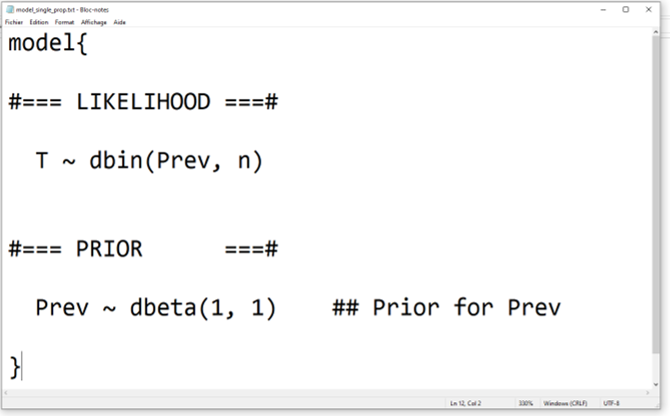
\includegraphics{Figures/Model_single_prop.png}
\caption{Text file with the model for estimating a single proportion.}
\end{figure}

\hypertarget{generating-initial-values}{%
\section{Generating initial values}\label{generating-initial-values}}

The initial value is the first value where each Markov chain will
start.\\
- You have to specify one initial value for each unknown parameter in
the model.\\
- If you decide to ran three Markov chains, you will need three
different sets of initial values.

For instance, in our preceding example we have one unknown parameter
(\emph{Prev}). If we were to run three Markov chains, we could generate
three sets of initial values for this parameter as follow. Of course,
the chosen values could be changed. In the case of a proportion, you can
specify any value between 0 and 1.

\begin{Shaded}
\begin{Highlighting}[]
\CommentTok{\#Initializing values for the parameter "Prev" for the 3 chains}
\NormalTok{inits }\OtherTok{\textless{}{-}} \FunctionTok{list}\NormalTok{(}
  \FunctionTok{list}\NormalTok{(}\AttributeTok{Prev=}\FloatTok{0.10}\NormalTok{),}
  \FunctionTok{list}\NormalTok{(}\AttributeTok{Prev=}\FloatTok{0.50}\NormalTok{),}
  \FunctionTok{list}\NormalTok{(}\AttributeTok{Prev=}\FloatTok{0.90}\NormalTok{)}
\NormalTok{  )}
\end{Highlighting}
\end{Shaded}

We know have a \texttt{R} object that I have called \emph{inits} and it
contains the values where each of the three Markov chains will start.

\hypertarget{running-a-model-in-jags}{%
\section{Running a model in JAGS}\label{running-a-model-in-jags}}

We now have the three elements that we needed: data, a model, and a set
of initial values. We can now use the \texttt{R2jags} library to run our
Bayesian analysis. The \texttt{R2jags} package provides an interface
from \texttt{R} to the JAGS software for Bayesian data analysis. JAGS
uses Markov Chain Monte Carlo (MCMC) to generate a sample from the
posterior distribution of the parameters.

The \texttt{R2jags} function that we will use for that is the
\texttt{jags()} function. Here are the arguments that we need to
specify:

\begin{itemize}
\tightlist
\item
  The dataset using \texttt{data=}\\
\item
  The text file containing the model written in JAGS code using
  \texttt{model.file=}.\\
\item
  The names of the parameters which should be monitored using
  \texttt{parameters.to.save=}.\\
\item
  The number of Markov chains using \texttt{n.chains=}. The default is
  3.\\
\item
  The sets of initial values using \texttt{inits=}. If inits is NULL,
  JAGS will randomly generate values.\\
\item
  The number of total iterations per chain (including burn-in; default:
  2000) using \texttt{n.iter=}.
\item
  The length of burn-in (i.e., number of iterations to discard at the
  beginning) using \texttt{n.burnin=}.
\item
  The thinning rate, which represent how many of the values sampled by
  the MCMC will be retained. The default is 5 (1 out of 5). Since there
  is no \emph{a priori} need for thinning, you can specify n.thin=1, in
  most situations.
\item
  The last argument \texttt{DIC=TRUE} or \texttt{DIC=FALSE} will
  determine whether to compute the deviance, pD, and deviance
  information criteria (DIC). These could sometimes be useful for model
  selection/comparison. We could leave that to \texttt{DIC=FALSE} since
  we will not be using these values in the workshop.
\end{itemize}

With the following code, we will create a \texttt{R} object called
\emph{bug.out}. This object will contains the results of running our
model, with the specified priors, using the available data, and the sets
of initial values that we have created. For this analysis, we have asked
to run 3 Markov chains, each for 6000 iterations and we discarded the
first 1000 iterations for each chain. Finally, we will monitor our only
unknown parameter, \emph{Prev} and nothing else.

\begin{Shaded}
\begin{Highlighting}[]
\FunctionTok{library}\NormalTok{(R2jags)}
\FunctionTok{library}\NormalTok{(coda)}

\CommentTok{\#Run the Bayesian model}
\NormalTok{bug.out }\OtherTok{\textless{}{-}} \FunctionTok{jags}\NormalTok{(}\AttributeTok{data=}\NormalTok{datalist,                             }\CommentTok{\#Specifying the R object containing the data}
               \AttributeTok{model.file=}\StringTok{"model\_single\_prop.txt"}\NormalTok{,         }\CommentTok{\#Specifying the .txt file containing the model}
               \AttributeTok{parameters.to.save=}\FunctionTok{c}\NormalTok{(}\StringTok{"Prev"}\NormalTok{),               }\CommentTok{\#Specifying the parameters to monitor. When \textgreater{}1 parameter, it will be a list, ex: c("Prev", "Se", "Sp")}
               \AttributeTok{n.chains=}\DecValTok{3}\NormalTok{,                                 }\CommentTok{\#Number of chains}
               \AttributeTok{inits=}\NormalTok{inits,                                }\CommentTok{\#Specifying the R object containing the initial values  }
               \AttributeTok{n.iter=}\DecValTok{6000}\NormalTok{,                                }\CommentTok{\#Specifying the number of iterations}
               \AttributeTok{n.burnin=}\DecValTok{1000}\NormalTok{,                              }\CommentTok{\#Specifying the number of iterations to remove at the begining}
               \AttributeTok{n.thin=}\DecValTok{1}\NormalTok{,                                   }\CommentTok{\#Specifying the thinning rate}
               \AttributeTok{DIC=}\ConstantTok{FALSE}\NormalTok{)                                  }\CommentTok{\#Indicating that we do not request the deviance, pD, nor DIC }
\end{Highlighting}
\end{Shaded}

\begin{verbatim}
## Compiling model graph
##    Resolving undeclared variables
##    Allocating nodes
## Graph information:
##    Observed stochastic nodes: 1
##    Unobserved stochastic nodes: 1
##    Total graph size: 4
## 
## Initializing model
\end{verbatim}

As you can see, we received a few messages. It looks good, don't you
think?

\hypertarget{model-diagnostic}{%
\section{Model diagnostic}\label{model-diagnostic}}

Before jumping to the results, you should first check:\\
- Whether the chains have converged,\\
- whether the burn-in period was long enough,\\
- Whether you have a large enough sample of values to describe the
posterior distribution with sufficient precision,\\
- Whether the Markov chains behaved well (mainly their
auto-correlation).

There are many diagnostic methods available for Bayesian analyses, but,
for this workshop, we will mainly use basic methods relying on plots.

Diagnostics are available when you convert your model output into a MCMC
object using the \texttt{as.mcmc()} function of the \texttt{mcmcplot}
library.

\begin{Shaded}
\begin{Highlighting}[]
\FunctionTok{library}\NormalTok{(mcmcplots)}
\NormalTok{bug.mcmc }\OtherTok{\textless{}{-}} \FunctionTok{as.mcmc}\NormalTok{(bug.out)          }\CommentTok{\#Converting the model output into a MCMC object (for diagnostic plots)}
\end{Highlighting}
\end{Shaded}

You can then use the \texttt{mcmcplot()} function on this newly created
MCMC object.

\begin{Shaded}
\begin{Highlighting}[]
\FunctionTok{mcmcplot}\NormalTok{(bug.mcmc, }\AttributeTok{title=}\StringTok{"Diagnostic plots"}\NormalTok{)        }\CommentTok{\#Asking for the diagnostic plots}
\end{Highlighting}
\end{Shaded}

When you do that, a HTML document will be created an your web browser
will automatically open it. Here is a snapshot of the HTML file in my
browser:

\begin{figure}
\centering
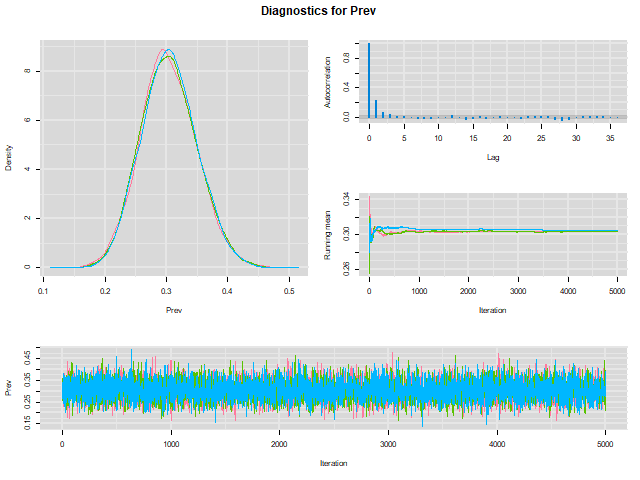
\includegraphics{Figures/Nice chains RM.png}
\caption{\textbf{Figure.} Diagnostic plots.}
\end{figure}

\hypertarget{convergence-and-burn-in}{%
\subsection{Convergence and burn-in}\label{convergence-and-burn-in}}

To check whether convergence of the Markov chains was obtained you can
inspect the ``running mean'' (right middle figure) and ``trace plot''
(the bottom figure) presenting the values that were picked by each chain
on each iteration. The different chains that you used (three in the
preceding example) will be overlaid on the trace plot. You should
inspect the trace plot to \textbf{evaluate whether the different chains
all converged in the same area}. If so, after a number of iterations
they should be moving in a relatively restricted area and this area
should be the same for all chains.

The plots above would be a good example of the trace plot of three
``nice'' Markov chains (lucky us!). In this preceding example, we can
see on the running mean plot that the chains started from different
initial values, but they very quickly converged (after less than a 1000
iterations) toward the same area. On the trace plot, we can see the
values that were stored after the burn-in period. The chains were then
moving freely within this limited area (thus sampling from the posterior
distribution).

We could conclude based on the trace plot that:\\
- The Markov chains did converged\\
- A short burn-in period of less than a 1000 iterations would have been
sufficient. Note that we will often use a longer burn-in (e.g., 5,000 or
even more) just to be sure and because it only costs a few more seconds
on your computer\ldots{}

Here is another example where two chains (the red and green) converged
in the same area, but a third one (the blue) also converged, but in a
different area. \textbf{We should be worry in such case}. We will see
later the reason for such behavior.
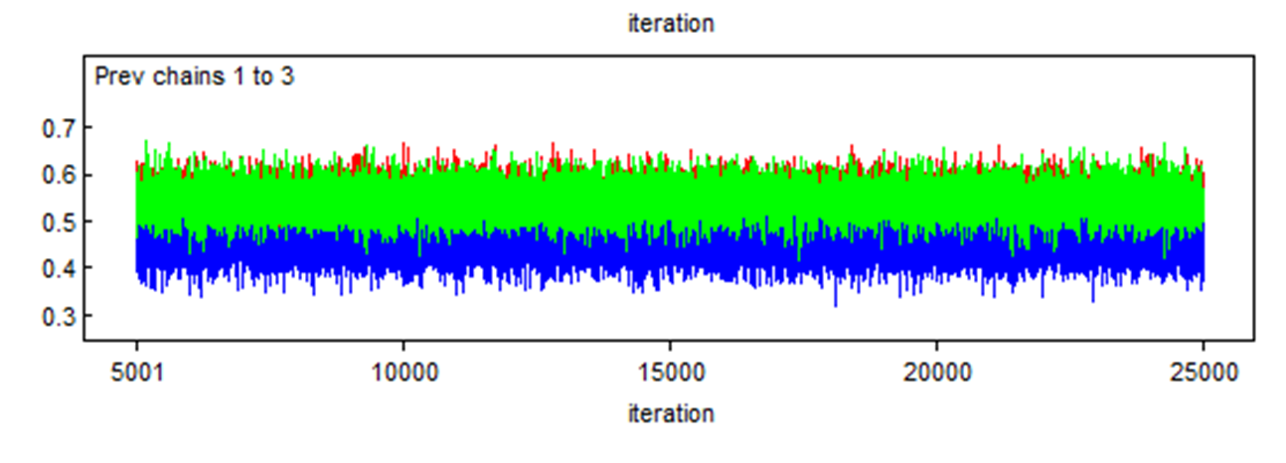
\includegraphics{Figures/2 nice 1 bad chain.png}

Finally, here is a last example with just one Markov chain and it
clearly did not converged, even after 25,000 iterations. \textbf{You
should be terrified by that!!! ;-)}.\\
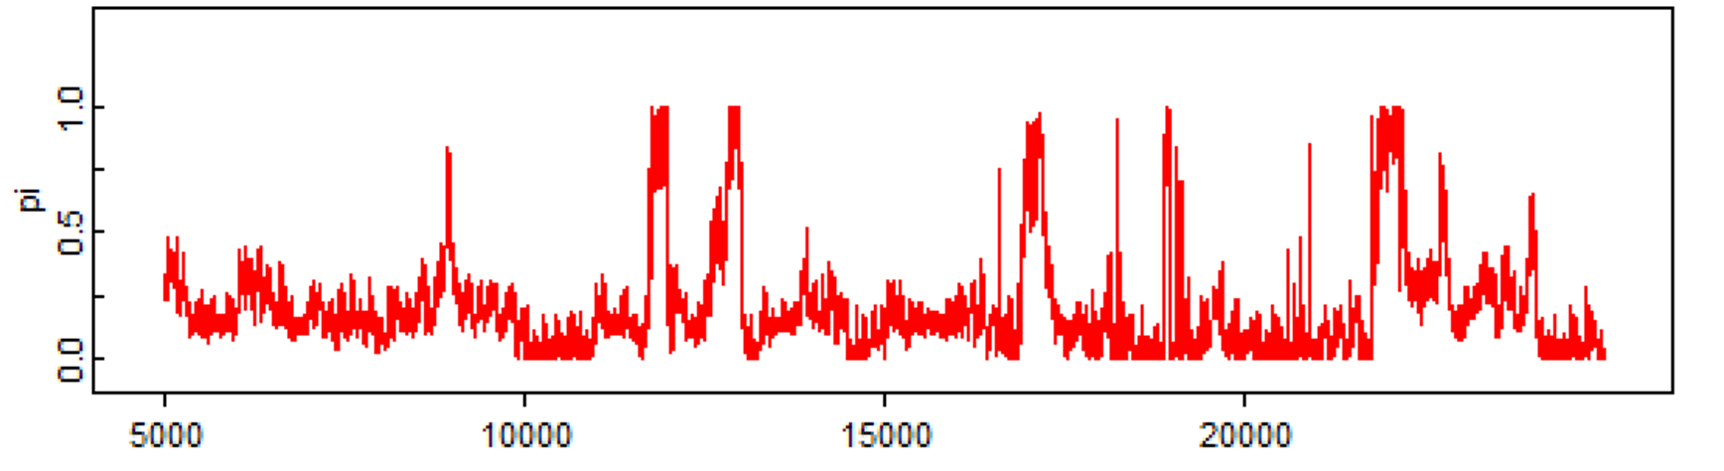
\includegraphics{Figures/non-conv chain.png}

\hypertarget{number-of-iterations}{%
\subsection{Number of iterations}\label{number-of-iterations}}

Next, you can inspect the posterior distributions to determine if you
have a large enough sample of independent values to describe with enough
precision the median estimate and the 2.5th and 97.5th percentiles. The
effective sample size (EES) takes into account the number of values
generated by the Markov chains \textbf{AND} whether these values were
auto-correlated, to compute the number of ``effective'' independent
values that are used to described the posterior distribution. Chains
that are auto-correlated will generate a smaller number of ``effective
values'' than chains that are not auto-correlated.

The \texttt{effectiveSize()} function of the \texttt{coda} library
provide a way to appraise whether you add enough iterations. In the
current example, we already created a \texttt{mcmc} object named
\texttt{bug.mcmc}. We can ask for the effective sample size as follow:

\begin{Shaded}
\begin{Highlighting}[]
\FunctionTok{effectiveSize}\NormalTok{(bug.mcmc)         }\CommentTok{\#Asking for the ESS}
\end{Highlighting}
\end{Shaded}

\begin{verbatim}
##     Prev 
## 9409.336
\end{verbatim}

So we see here that, despite having stored 3 times 5,000 values (15,000
values), we have the equivalent of a bit more than 9,000 independent
values. What to do with this information? Well, you could, for instance,
decide on an arbitrary rule for ESS (say 10,000 values) and then adapt
the length of the chains to achieve such an ESS (for each of the
selected parameters, because the effective sample sizes will not be the
same for all parameters).

\hypertarget{auto-correlation}{%
\subsection{Auto-correlation}\label{auto-correlation}}

Remember, a feature of Markov chains is to have some auto-correlation
between two immediately subsequent iterations and then a correlation
that quickly goes down to zero (i.e., they have a short memory). The
auto-correlation plot can be used to assess if this feature is
respected.

From our previous example (check the upper right figure in the plot
below), it seems that it is the case.\\
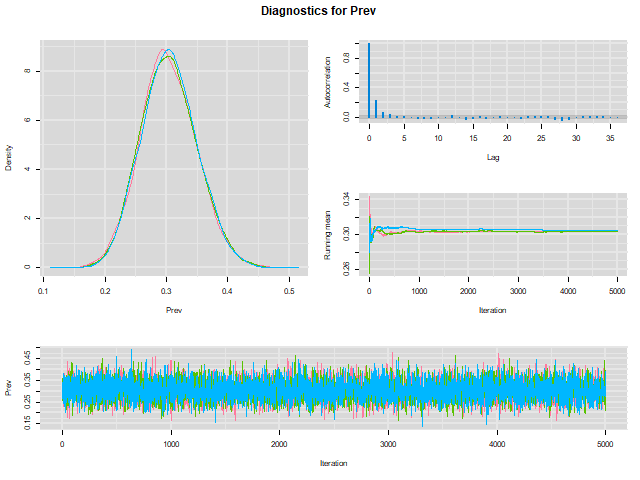
\includegraphics{Figures/Nice chains RM.png}

Here is another example that should be worrying.\\
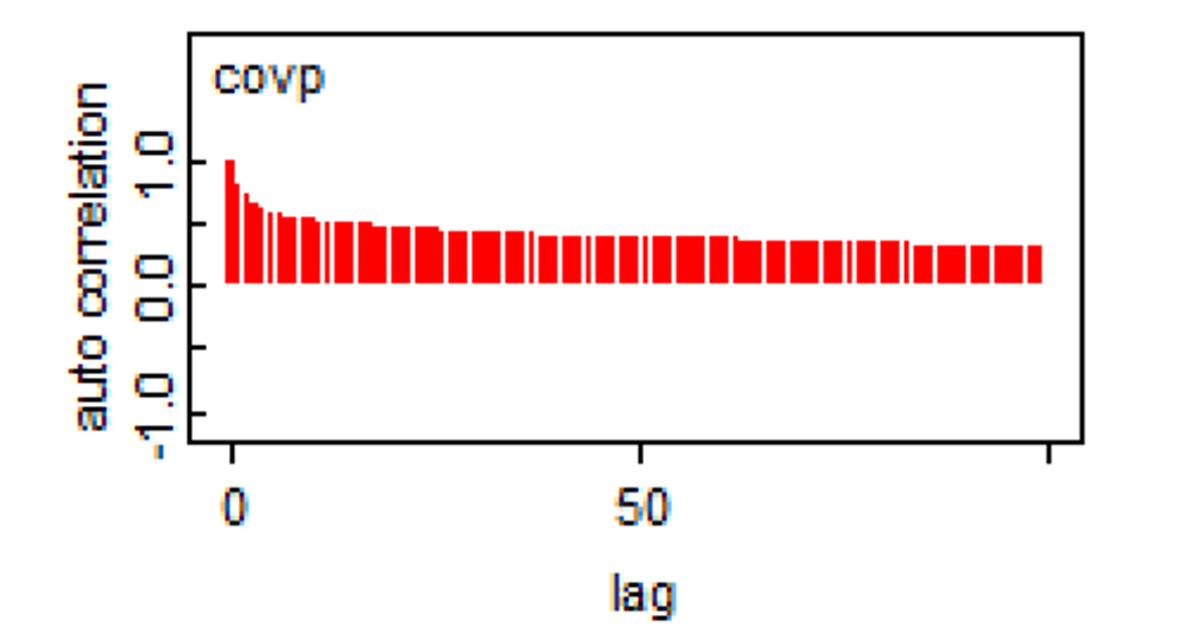
\includegraphics{Figures/Autocor bad.png}

When such a behavior is observed, running the chains for more iterations
will help achieve the desire ESS. In some situations, specifying
different priors (i.e., increasing the amount of information in priors)
may also help.

\hypertarget{getting-our-estimates}{%
\section{Getting our estimates}\label{getting-our-estimates}}

Now, if you are happy with the behavior of your Markov chains, the
number of iterations, and burn-in period, you can summarize your results
(i.e., report the median, 2.5th and 97.5th percentiles) very easily with
the \texttt{print()} function. Below, I have also indicated
\texttt{digits.summary=3} to adjust the precision of the estimates that
are reported (the default is 1).

\begin{Shaded}
\begin{Highlighting}[]
\FunctionTok{print}\NormalTok{(bug.out,                  }\CommentTok{\#Asking to see the mean, median, etc of the unknown parameters that were monitored}
      \AttributeTok{digits.summary=}\DecValTok{3}\NormalTok{)         }\CommentTok{\#Requiring a precision of 3 digits}
\end{Highlighting}
\end{Shaded}

\begin{verbatim}
## Inference for Bugs model at "model_single_prop.txt", fit using jags,
##  3 chains, each with 6000 iterations (first 1000 discarded)
##  n.sims = 15000 iterations saved
##      mu.vect sd.vect  2.5%   25%   50%   75% 97.5%  Rhat n.eff
## Prev   0.304   0.045 0.219 0.273 0.302 0.334 0.397 1.001 15000
## 
## For each parameter, n.eff is a crude measure of effective sample size,
## and Rhat is the potential scale reduction factor (at convergence, Rhat=1).
\end{verbatim}

Here you see that the median \emph{Prev} estimate (95CI) was (after
rounding off) 0.30 (0.22, 0.40).

You can also ask for plotting the \emph{bug.mcmc} object that you have
created using the \texttt{plot()} function. It would produce the trace
plot and a density plot presenting the posterior distributions of each
unknown parameter.

\begin{Shaded}
\begin{Highlighting}[]
\FunctionTok{plot}\NormalTok{(bug.mcmc)              }\CommentTok{\#Asking for trace plot and plots of prior and posterior distributions}
\end{Highlighting}
\end{Shaded}

\begin{figure}
\centering
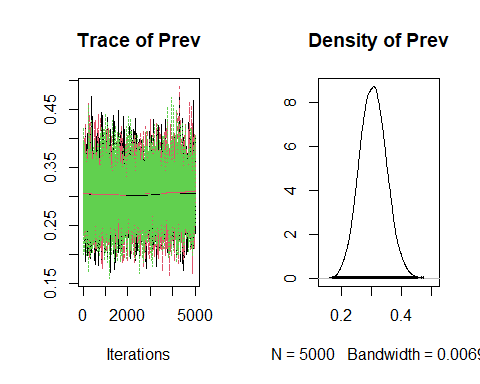
\includegraphics{_main_files/figure-latex/unnamed-chunk-25-1.pdf}
\caption{Trace plot and density plot produced using the plot()
function.}
\end{figure}

If you prefer to work on your own plots, note that all the values
sampled from your posterior distributions were stored in the
\emph{bug.out} object that you have created. If you inspect the
\emph{bug.out} object, you will notice an element named
\emph{BUGSoutput}, inside this element, there is another object named
\emph{sims.list}, within this \emph{sims.list}, there is an element
named \emph{Prev}. As you can see below, this element is made of a list
of 15000 values. This correspond to the 5000 values sampled
(1/iteration) by each Markov chain (3 chains) for the unknown parameter
\emph{Prev}. \textbf{So this element is simply all the sampled values
assembled together}.

\begin{figure}
\centering
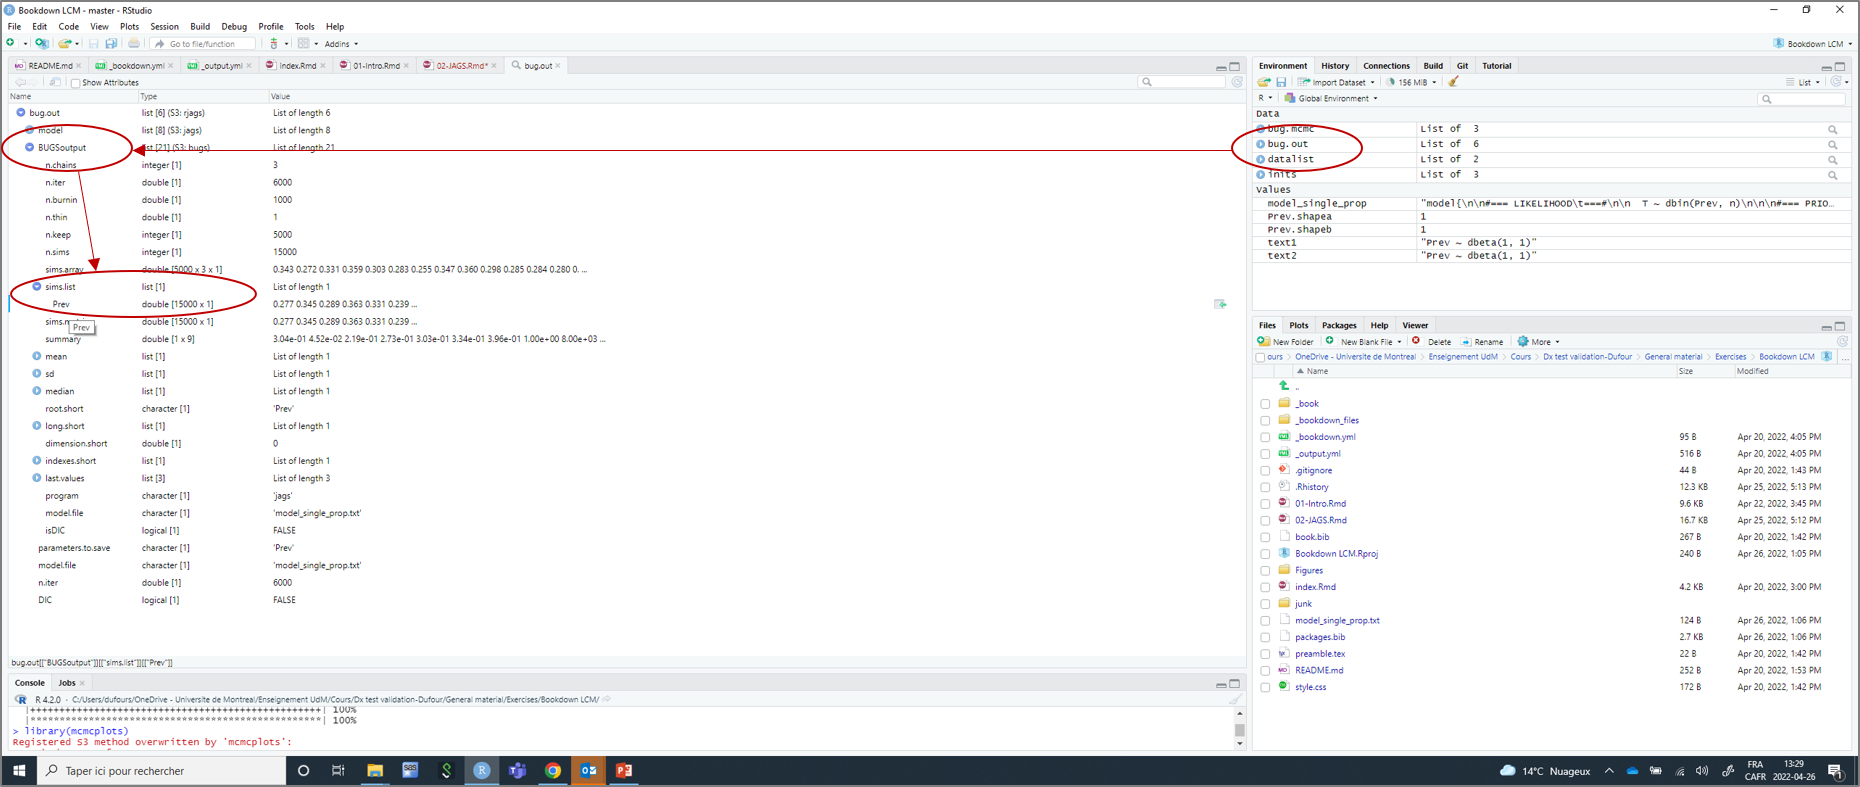
\includegraphics{Figures/sims list.png}
\caption{sims.list object located in the \emph{bug.out} output.}
\end{figure}

You could use this element, for instance, to plot together the prior and
posterior distributions on a same figure. On the figure below, the prior
distribution is not obvious, it is the flat dashed red line just above
the x axis (remember, we used a flat prior for \emph{Prev}).

\begin{Shaded}
\begin{Highlighting}[]
\CommentTok{\#Plot the posterior distribution}
\FunctionTok{plot}\NormalTok{(}\FunctionTok{density}\NormalTok{(}\AttributeTok{x=}\NormalTok{bug.out}\SpecialCharTok{$}\NormalTok{BUGSoutput}\SpecialCharTok{$}\NormalTok{sims.list}\SpecialCharTok{$}\NormalTok{Prev),      }\CommentTok{\#Indicating variable to plot}
     \AttributeTok{main=}\StringTok{"Disease prevalence"}\NormalTok{,                         }\CommentTok{\#Title for the plot}
     \AttributeTok{xlab=}\StringTok{"Prevalence"}\NormalTok{, }\AttributeTok{ylab=}\StringTok{"Density"}\NormalTok{,                 }\CommentTok{\#x and y axis titles}
\NormalTok{     )}

\CommentTok{\#plot the prior distribution}
\FunctionTok{curve}\NormalTok{(}\FunctionTok{dbeta}\NormalTok{(x, }\AttributeTok{shape1=}\NormalTok{Prev.shapea, }\AttributeTok{shape2=}\NormalTok{Prev.shapeb), }\AttributeTok{from=}\DecValTok{0}\NormalTok{, }\AttributeTok{to=}\DecValTok{1}\NormalTok{,          }\CommentTok{\#Plotting the corresponding prior distribution}
      \AttributeTok{lty=}\DecValTok{2}\NormalTok{,                                                                   }\CommentTok{\#Asking for a dashed line pattern}
      \AttributeTok{col=}\StringTok{"red"}\NormalTok{,                                                               }\CommentTok{\#Asking for a red line  }
      \AttributeTok{add=}\ConstantTok{TRUE}\NormalTok{)                                                                }\CommentTok{\#Asking to add this plot to the preceding one}
\end{Highlighting}
\end{Shaded}

\begin{figure}
\centering
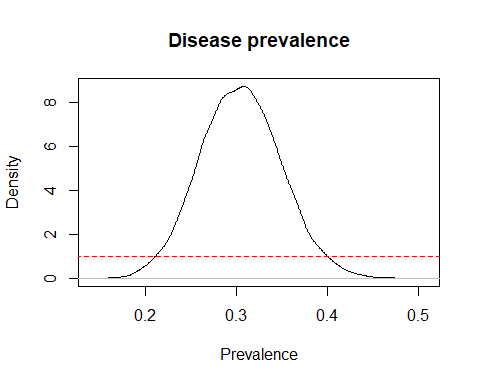
\includegraphics{_main_files/figure-latex/unnamed-chunk-26-1.pdf}
\caption{Prior (dashed red line) and posterior (full black line)
distribution of the prevalence of disease.}
\end{figure}

\hypertarget{exercise-1---proportions}{%
\chapter{Exercise 1 - Proportions}\label{exercise-1---proportions}}

\hypertarget{data}{%
\section{Data}\label{data}}

The data used for the following exercises came from a study aiming at
estimating diagnostic accuracy of a milk pregnancy associated
glycoprotein (\textbf{PAG}) ELISA and of transrectal ultrasonographic
(\textbf{US}) exam when used for determining pregnancy status of
individual dairy cows 28 to 45 days post-insemination. In that study,
the new test under investigation was the PAG test and US was used for
comparison, but was considered as an imperfect reference test.

In the original study, data from 519 cows from 18 commercial dairy herds
were used. For the following exercises, the dataset was modified so that
we have data from 519 cows from 3 herds (i.e., the data from 16 herds
were collapsed together so they appear to be from one large herd). Note
that there are some cows with missing values for one of the tests, so we
will not always work with 519 cows. The complete original publication
can be found here:
\href{https://www.sciencedirect.com/science/article/pii/S016758771630527X?casa_token=jmHY9HiOdEYAAAAA:kGdiIujRzrAQjjFRbGqtUxIBalDGvXllp6ja9w4T2s6c7yPbgc0asnak79bJ5GWWXI8InhCg0sg}{Dufour
et al., 2017}.

The dataset \emph{Preg.xlsx} contains the results from the study.
However, \textbf{for the exercises we will always simply used the
cross-tabulated data and these will be already organized for you and
presented at the beginning of each exercise}. The dataset is still
provided so you can further explore additional comparisons. The list of
variables in the \emph{Preg.xlsx} dataset are described in the table
below.

\textbf{Table}. List of variables in the \emph{Preg.xlsx} dataset.

\begin{longtable}[]{@{}
  >{\raggedright\arraybackslash}p{(\columnwidth - 4\tabcolsep) * \real{0.1505}}
  >{\raggedright\arraybackslash}p{(\columnwidth - 4\tabcolsep) * \real{0.5054}}
  >{\raggedright\arraybackslash}p{(\columnwidth - 4\tabcolsep) * \real{0.3441}}@{}}
\toprule
\begin{minipage}[b]{\linewidth}\raggedright
\textbf{Variable}
\end{minipage} & \begin{minipage}[b]{\linewidth}\raggedright
\textbf{Description}
\end{minipage} & \begin{minipage}[b]{\linewidth}\raggedright
\textbf{Range}
\end{minipage} \\
\midrule
\endhead
Obs & An observation unique ID number & 1 to 519 \\
Herd & Herd ID number & 1 to 3 \\
Cow & Cow ID number & NA \\
T1\_DOP & Number of days since insemination at testing & 28 to 45 \\
PAG\_DX & Results from the PAG test & 0 (not pregnant); 1 (pregnant) \\
US\_DX & Results from the ultrasound test & 0 (not pregnant); 1
(pregnant) \\
TRE\_DX & Results from the transrectal exam (TRE) test & 0 (not
pregnant); 1 (pregnant) \\
\bottomrule
\end{longtable}

\hypertarget{questions}{%
\section{Questions}\label{questions}}

In the study, we had the following proportion of apparently pregnant
cows (based on the US exam).

\textbf{257 US+/497 exams}

Open up the \texttt{R} project for Exercise 1 (i.e., the R project file
named \emph{Exercise 1.Rproj}).

In the Exercise 1 folder, you will find partially completed \texttt{R}
scripts. To answer the questions, try to complete the missing parts
(they are highlighted by a \textbf{\#TO COMPLETE\#} comment). We also
provided complete \texttt{R} scripts, but try to work it out on your own
first!

\textbf{1. Start from the partially completed \emph{Question 1.R}
\texttt{R} script located in Exercise 1 folder.} What would be the
proportion of pregnant cows? Use a Bayesian approach to compute that
proportion and a credible interval (\textbf{CI}). For this first
computation, assume that you have no prior knowledge on the expected
proportion of pregnant cows in a Canadian herd. Run three Markov chains
with different sets of initial values. Look at the trace plot. Do you
think convergence was achieved? Do you need a longer burn-in period? Are
all 3 chains converging in the same space? Compute the effective sample
size (\textbf{ESS}), do you feel that number of iterations was
sufficient to describe the posterior distribution with enough precision?
What about auto-correlation of the Markov chains, any issues there?

\textbf{2.} If you were to compute a Frequentist estimate with 95\% CI,
would it differ a lot from your Bayesian estimates? Why? As a refresher,
the formula for a Frequentist 95\%CI for a proportion is below (where
\emph{P} is the actual observed proportion and \emph{n} is the
denominator for that proportion):

\(95CI=P \pm 1.96* \sqrt{\frac{P*(1-P)}{n}}\)

\textbf{3. Start from the \texttt{R} script that you completed in
Question 1.} In the literature, you saw a recent study conducted on 30
Canadian herds and reporting an expected pregnancy prevalence of 42\%
with 97.5\% percentile of 74\%. What kind of distribution could you use
to represent this information? Use these information as a pregnancy
prevalence prior distribution. Are your results very different?

\textbf{4. Start from the partially completed \emph{Question 4.R}
\texttt{R} script located in Exercise 1 folder.} When comparing PAG to
TUS results for the whole dataset, you got the following 2x2 table.

\textbf{Table.} Cross-classified results of the PAG and TUS tests.

\begin{longtable}[]{@{}llll@{}}
\toprule
& \textbf{TUS+} & \textbf{TUS-} & \textbf{Total} \\
\midrule
\endhead
\textbf{PAG+} & 255 & 21 & 276 \\
\textbf{PAG-} & 2 & 219 & 221 \\
\textbf{Total} & 257 & 240 & 497 \\
\bottomrule
\end{longtable}

Assuming that TUS is a gold-standard test could you compute PAG
sensitivity (\textbf{Se}) and specificity (\textbf{Sp})? Use vague
priors for PAG Se and Sp since it is the first ever study on this topic
(i.e., you do not have any prior knowledge on these unknown parameters).

\hypertarget{answers}{%
\section{Answers}\label{answers}}

\textbf{1.} What would be the proportion of pregnant cows? Use a
Bayesian approach to compute that proportion and a credible interval
(\textbf{CI}). For this first computation, assume that you have no prior
knowledge on the expected proportion of pregnant cows in a Canadian
herd. Run three Markov chains with different sets of initial values.
Look at the trace plot. Do you think convergence was achieved? Do you
need a longer burn-in period? Are all 3 chains converging in the same
space? Compute the effective sample size (\textbf{ESS}), do you feel
that number of iterations was sufficient to describe the posterior
distribution with enough precision? What about auto-correlation of the
Markov chains, any issues there?

\textbf{Answer:} I chose to run a model with 3 chains of 10,000
iterations each (11,000 iterations minus a burn-in of 1,000). I have
obtained the following diagnostic plots:

\begin{figure}
\centering
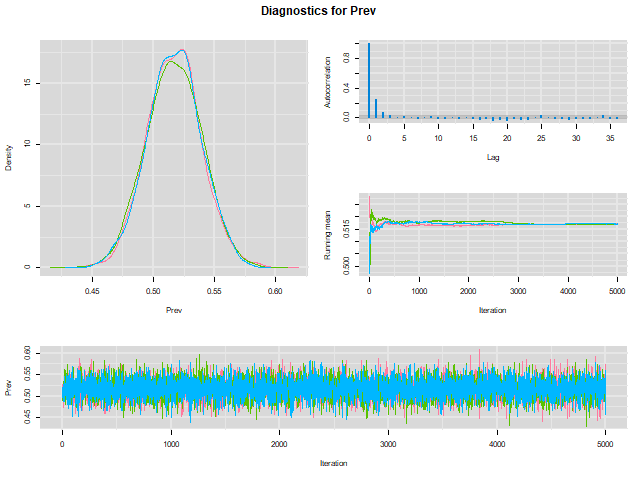
\includegraphics{Figures/Ex1_Q1_Dx.png}
\caption{Diagnostic plot}
\end{figure}

Convergence of the 3 chains was achieved, all three chains appear to be
moving in the same space (see trace plot). The 1,000 iterations burn-in
period is probably more than needed for this very simple problem.
Autocorrelation plot is just perfect with correlation declining very
rapidly close to zero at lag of 1! The effective sample size for the
\emph{Prev} parameter is \textgreater17,000 values. So, plenty of
precision to report the median and 2.5th and 97.5th percentiles.

The median pregnancy prevalence estimate (95\% CI) was 51.7\% (47.3,
56.1).

\textbf{2.} If you were to compute a frequentist estimate with 95\% CI,
would it differ a lot from your Bayesian estimates? Why?

\textbf{Answer:} It should not differ much from the Bayesian median
estimate and 95CI because these latter estimates were generated using
vague priors. In such cases, Bayesian and Frequentist estimates should
be quite similar. Actually, if we use the Frequentist formula for
computing 95CI and the observed data (i.e., 257/497) we get:

\(P = 257/497 = 0.517\)

\(95CI=0.517 \pm 1.96* \sqrt{\frac{0.517*(1-0.517)}{497}} = 0.517 \pm 0.044\)

Thus, we have a Frequentist estimated proportion of 51.7\% with a
Frequentist 95 CI of 47.3 to 56.1 (virtually unchanged compared to the
Bayesian estimates).

\textbf{3.} In the literature, you saw a recent study conducted on 30
Canadian herds and reporting an expected pregnancy prevalence of 42\%
with 97.5\% percentile of 74\%. What kind of distribution could you use
to represent this information? Use these information as a pregnancy
prevalence prior distribution. Are your results very different?

\textbf{Answer:} A beta(4.2, 5.4) distribution would have a mode of 0.42
and a 97.5th percentile of 0.74. Using this information as prior, I get
a prevalence of pregnancy of 51.6\% (95 CI: 47.2, 55.8). Actually, we
observe very little difference between the models using vague \emph{vs.}
informative priors. This is because this informative prior contains only
the equivalent of 10 observations \((4.2+5.4)\). In the dataset, there
are 497 cows. Therefore, the estimation process is still mainly driven
by our dataset.

\textbf{4.} When comparing PAG to TUS results for the whole dataset, you
got the following 2x2 table. Assuming that TUS is a gold-standard test
could you compute PAG sensitivity (\textbf{Se}) and specificity
(\textbf{Sp})? Use vague priors for PAG Se and Sp since it is the first
ever study on this topic (i.e., you do not have any prior knowledge on
these unknown parameters).

\textbf{Answer:} A sensitivity or a specificity are, similarly to a
prevalence, simple proportions. Sensitivity is simply the number of test
positive among the number of true positive. We have data for these in
the 2x2 table. If we assume that \emph{US} is a gold-standard test, than
number of true positive cows is 257. And 255 of them tested positive to
the \emph{PAG} test. Similarly, the specificity is simply the number of
test negative among the number of true negative. From the 2x2 table, the
number of true negative cows was 240 and 219 of them tested negative to
the \emph{PAG} test. The likelihood functions (one for each parameter in
this case) linking the unknown parameters (\emph{Se} and \emph{Sp}) to
these observed data would be:

\(Test+ \sim dbin(Se, True+)\)

\(Test- \sim dbin(Sp, True-)\)

Using vague beta(1, 1) priors on the \emph{Se} and \emph{Sp}, I got an
estimated \emph{Se} of 99.0\% (95 CI: 97.3, 99.8) and a \emph{Sp} of
91.0\% (95CI: 87.0, 94.2). \textbf{But be cautious with these numbers.}
We know very well that an \emph{US} exam is not a perfect diagnostic
test for pregnancy in dairy cows. With the current approach, we are
attributing all disagreements between tests to a failure of the
\emph{PAG} test\ldots{} But it could be the \emph{US} test that was
wrong in many instances. Moreover, animals for which the two tests
agreed could still be misdiagnosed as pregnant or open, but by both
tests (i.e., a failure of the \emph{PAG} \textbf{AND} the \emph{US}
tests). We wil see in the next parts of the course how to account for
the fact that neither of the tests are gold-standards.

\backmatter
\end{document}
